
%Para melhor utilização da ferramenta, utilize o pdfLaTeX+MakeIndex+BibTeX%
\documentclass[article,12pt,oneside,a4paper,english,brazil]{unifil}

% IMPORTS
\usepackage{placeins}
\usepackage{pgfgantt}

\DeclareUnicodeCharacter{00A0}{ }

% Caso queira usar um diretório diferente pra imagem, tire o comentário da proxima linha 
% \graphicspath{ {/home/hug/MonografeArq/}}
\titulo{Um Estudo Econômico-Computacional Aplicado Sobre Criptoativos \\ 
\fontsize{12}{14}\selectfont An Applied Economic-Computational Study
On Cryptoassets}
\autor{Heber José da Silva Junior\thanks{Centro Universitário Filadélfia de Londrina - UniFil}
\\Mario Henrique Akihiko da Costa Adaniya\thanks{Centro Universitário Filadélfia de Londrina - UniFil}}
\instituicao{Centro Universitário Filadélfia}
\local{Londrina}
\predate{}
\postdate{}
\date{}

\makeatletter
\let\@fnsymbol\@arabic
\makeatother

\usepackage{caption}
\captionsetup[figure]{slc=off}

\usepackage{titling}
\setlength{\droptitle}{-3cm}
\preauthor{\begin{flushright}
\large \lineskip 0.5em%
}
\postauthor{\end{flushright}}

\usepackage{graphicx}
\usepackage{titlesec}
\titleformat{\section}
{\normalfont\fontsize{14}{15}\bfseries}{\thesection}{1em}{}

\SingleSpacing

\begin{document}
\frenchspacing
\maketitle 
\normalsize

\fontsize{10}{1}\selectfont
\section*{Resumo}
Nos últimos anos, as criptomoedas têm conquistado seu caminho no cenário financeiro global, trazendo uma nova maneira na realização de transações econômicas. A ascensão das moedas digitais como o \textit{Bitcoin} e \textit{Ethereum} trouxeram consigo não apenas uma revolução na tecnologia financeira, mas também uma onda de especulação, debate e inovação. No entanto, além do seu potencial como veículo de investimento e meio de troca, o mundo dos criptoativos abre portas também para a propósitos educacionais. Este artigo explora a possibilidade e a tecnologia necessária no desenvolvimento de um criptoativo educacional, voltado a refinar a maneira em que as pessoas aprendem os princípios fundamentais da ciência econômica e financeira. Este projeto se utiliza das bases das moedas digitais, suas tecnologias empregadas e seu impacto sobre a economia tradicional, se apoiando também na definição do dinheiro sob a visão dos autores presentes na Escola Austríaca de Economia.\\
\vspace{\onelineskip} \\
\noindent
\textbf{Palavras-chave}: Tecnologia financeira; Economia; \textit{Blockchain}; \textit{Bitcoin}; Educação financeira; Criptoativos; \textit{DeFi}.



\section*{Abstract}
\begin{otherlanguage*}{english}
%resumo em ingles%
In recent years, cryptocurrencies have burst onto the global financial scene, bringing with them a new way of conducting economic transactions. The rise of digital currencies such as bitcoin and ethereum has not only revolutionized financial technology, but also sparked a wave of speculation, debate, and innovation. But beyond its potential as an investment vehicle and medium of exchange, the world of cryptoassets also opens doors for educational purposes. This article explores the possibility and the technology required to develop an educational cryptoasset aimed at refining the way people learn the basic principles of economics and finance. This project uses the fundamentals of digital currencies, their technologies and their impact on the traditional economy, and also draws on the definition of money from the point of view of the authors of the Austrian School of Economics.\\
\vspace{\onelineskip}\\
\noindent
\textbf{Keywords}: Financial technology; Economics; \textit{Blockchain}; \textit{Bitcoin}; Financial education; Cryptoassets; \textit{DeFi}
\end{otherlanguage*}
\clearpage

%texto%
\textual
\fontsize{12}{7}\selectfont
\begin{Spacing}{1.5}

\section*{INTRODUÇÃO}

Os criptoativos, também conhecidos como criptomoedas ou moedas digitais, são representações digitais de valor que utilizam criptografia para garantir transações seguras e controlar a criação de novas unidades \cite{Yetmar2023}. Ao contrário das moedas governamentais tradicionais, os criptoativos operam em redes descentralizadas, geralmente baseadas em tecnologia de \textit{Blockchain}, onde a validação das transações é realizada pelos próprios participantes da rede através de um consenso distribuído. Este ambiente transparente, seguro e descentralizado existe graças a arquiteturas de \textit{software} complexas e dedicadas ao propósito de escalabilidade, segurança e autonomia do ativo. Diante da versatilidade dos criptoativos, este projeto de pesquisa visa esclarecer o entendimento popular dos criptoativos enquanto expõe uma análise técnica e econômica do mesmo. 

Na seção \ref*{sec:bitcoin} utilizamos do \textit{Bitcoin} como exemplo, expomos o contexto de aplicação deste ativo, seu posicionamento sobre o dinheiro tradicional e como podemos utilizar do ambiente das criptos para buscar independência monetária. É apresentado também a tecnologia de encadeamento e rede em que o Bitcoin atua — a \textit{Blockchain}, a tecnologia Prova de Trabalho, ou \textit{Proof of work}, utilizada como validador de novos blocos e a técnica utilizada na assinatura de transações dentro da \textit{Blockchain} — a criptografia de chave pública e privada.

Pela seção \ref*{sec:austriaca} são adotadas as definições de dinheiro, economia e capital da Escola Austríaca de Economia. Será utilizado dos conceitos financeiros para definir quão bem o criptoativo consegue servir as atividades econômicas.

Durante a seção \ref*{sec:dinheiro} é feita uma revisão do livro ``\textit{Bitcoin}, A Moeda Na Era Digital'' do mestre brasileiro em economia Fernando Ulrich. Neste livro o autor também revisa o posicionamento da Escola Austríaca de Economia diante do conceito de dinheiro e moeda, traz contexto histórico sobre o desenvolvimento do \textit{Bitcoin} e defende a utilização do criptoativo como moeda de troca legítimo.


Por fim, no capítulo \ref*{sec:educativo}, propomos a ideia do desenvolvimento de uma criptomoeda capaz de conteinerizar e abstrair os conceitos básicos do ensino de economia, provendo autonomia para professores simularem ambientes econômicos. Assim demonstrando e aplicando o conhecimento teórico da ciência financeira.

% PROBLEMATICA

Embora as criptomoedas tenham ganhado destaque, a compreensão abrangente de seu estado técnico atual permanece fragmentada. Esta falta de clareza popular diante do contexto de criptoativos torna o conceito menos palatável à aceitação pública da tecnologia. Embora compreendível a baixa adesão popular a tal tecnologia, é possível estipular melhorias de qualidade de vida diante da população passando despercebidas.

Como conceito, as finanças descentralizadas nasceram visando denunciar as consequências sofridas pela população devido ao mal uso governamental do curso forçado das suas respectivas moedas. A ideia de retirar a manipulação central do dinheiro cria impeditivos físicos ao ativo de sofrer anomalias econômicas como a inflação, por exemplo, visto que o comportamento de escassez da moeda é absoluto (no caso do \textit{Bitcoin}).

Conforme o mestre em desenvolvimento econômico Pedro Lopes Marinho, em 2001, devido o início da Primeira Guerra Mundial, o sistema monetário padrão-ouro foi mundialmente abolido enquanto governos financiavam os gastos militares a partir da emissão de moedas. Uma vez que o lastro em metal na moeda foi abandonado, o maior impeditivo a impressão deliberada de dinheiro — e posteriormente inflação — foi deixado de lado.

A ideia da economia estar sob o controle absoluto governamental implica que todo o trabalho, tempo, esforço e riqueza de uma população está a uma ordem de distância de ser descartada por mal uso estatal da sua moeda. 

Assim que as finanças descentralizadas tomam seu devido foco. Uma vez oferecendo independência, autonomia, transparência e integridade dos seus protocolos, as moedas digitais podem garantir que o poder e a responsabilidade do dinheiro estão apenas sob quem os detém, seguindo a máxima popular do ambiente cripto ``Minhas chaves, minhas moedas''.

% Limitações do trabalho

O projeto de pesquisa passa pela limitação de que, no estado atual de atividade entre meio destes ativos, o lançamento de novas moedas digitais são extremamente frequentes, gerando constante necessidade de reindexação da funcionalidade e atuação de cada nova moeda.


% \section*{METODOLOGIA DE PESQUISA}
\chapter{Metodologia de Pesquisa}

% Metodologia a ser utilizada para verificar a hipótese, com justificativa.









% \section*{ESTADO DA ARTE}
\chapter{Estado da Arte}
O estudo dos criptoativos, frequentemente referidos como criptomoedas, emergiu como uma área interdisciplinar que engloba finanças, economia, ciência da computação, direito e outras disciplinas correlatas. O estado da arte nesta área é caracterizado por avanços tecnológicos inovadores, desafios regulatórios complexos, crescente adoção institucional e individual, e um cenário de rápida evolução e inovações contínuas.

% O estado da arte dos criptoativos é marcado por uma confluência de avanços tecnológicos, desenvolvimentos regulatórios, crescente adoção e contínuas inovações. À medida que a tecnologia blockchain evolui e a regulamentação se torna mais clara, os criptoativos têm o potencial de transformar significativamente o panorama financeiro global, introduzindo novos paradigmas de descentralização, segurança e eficiência. A pesquisa contínua e a colaboração entre setores serão essenciais para navegar os desafios e aproveitar as oportunidades apresentadas por esta tecnologia emergente.

\section{Tecnologia}
A seguir consta as principais tecnologias aplicadas ao ambiente das finanças distribuídas, será apresentado brevemente seus respectivos contextos e utilizações.

\section*{\textit{Blockchain} e Tecnologia de Registro Distribuído (DLT)}

A \textit{blockchain}, a partir da Tecnologia de Registro Distribuído (DLT), é o alicerce sobre o qual a maioria dos criptoativos é construída. Sua estrutura descentralizada  permite a verificação e registro de transações por uma rede distribuída de nós, assegura características fundamentais como imutabilidade, transparência e resistência à censura \cite{Nakamoto2009}. Além disso, protocolos de consenso como \textit{Proof of Work (PoW)} e \textit{Proof of Stake (PoS)} são cruciais para a segurança e eficiência das redes \textit{blockchain}.

\section*{Contratos Inteligentes}

Contratos inteligentes \textit{(smart contracts)} são programas autoexecutáveis que operam quando condições predefinidas são atendidas. Introduzidos pela plataforma \textit{Ethereum} \cite{buterin2013ethereum}, esses contratos têm o potencial de automatizar e desintermediar uma vasta gama de transações e processos contratuais, desde serviços financeiros até cadeias de suprimentos. A segurança e a flexibilidade proporcionadas pelos contratos inteligentes incentivam a criação de Aplicações Descentralizadas \textit{(DApps)}, que operam em redes \textit{blockchain} sem necessidade de intermediários confiáveis.

\section*{Interoperabilidade}

Um dos desafios técnicos significativos é a interoperabilidade entre diferentes blockchains. Projetos como \textit{Polkadot} \cite{wood2016polkadot} e Cosmos \cite{kwon2016cosmos} estão na vanguarda do desenvolvimento de soluções que permitem a comunicação e a interação entre diversas redes \textit{blockchain}. Esta interoperabilidade é essencial para a criação de um ecossistema de criptoativos mais integrado e funcional, onde ativos e informações podem ser transferidos de maneira segura e eficiente entre diferentes plataformas.

\section{Regulamentação}

Nesta seção é documentada as respostas de maior incisão no ambiente cripto por parte do âmbito governamental. 

\section*{Panorama Regulatório}

O cenário regulatório dos criptoativos é altamente diversificado e dinâmico. Países como Suíça e Singapura têm adotado abordagens regulatórias favoráveis, criando ambientes propícios para inovação e atração de investimentos \cite{zohar2015bitcoin}. Em contraste, nações como China e Índia têm implementado restrições rigorosas ao uso e comércio de criptoativos, citando preocupações com a estabilidade financeira e a proteção ao consumidor \cite{auer2018regulating}.

\section*{Iniciativas Globais}

Instituições internacionais, como o \textit{Financial Action Task Force (FATF)}, estão desenvolvendo diretrizes para mitigar os riscos associados aos criptoativos, como a lavagem de dinheiro e o financiamento do terrorismo \cite{fatf2019guidance}. A União Europeia, com sua proposta de Regulamento de Mercados de Criptoativos (MiCA), afirma buscar estabelecer um quadro regulamentar abrangente que ofereça proteção aos investidores enquanto promove a inovação no setor \cite{european2020proposal}.

\section{Adoção}

Nesta seção é constatado o âmbito popular e empresarial diante da adoção do uso de criptoativos em seu cotidiano.

\section*{Adoção Institucional}

A adoção de criptoativos por instituições financeiras e empresas de grande porte tem crescido substancialmente. Empresas como \textit{Tesla} e \textit{MicroStrategy} têm incorporado Bitcoin em suas estratégias de reserva de tesouraria, sinalizando uma crescente aceitação dos criptoativos como reserva de valor \cite{bouri2017hedge}. Além disso, grandes instituições financeiras estão desenvolvendo produtos de investimento baseados em criptoativos, como fundos negociados em bolsa (ETFs) e contratos futuros.

\section*{Adoção pelo Consumidor}

A adoção de criptoativos por consumidores está aumentando, impulsionada pela facilidade de acesso através de carteiras digitais e plataformas de negociação \cite{kondor2014do}. Serviços de pagamento como \textit{PayPal} e \textit{Square} permitem a compra, venda e uso de criptomoedas, tornando-as mais acessíveis ao público. Esta crescente adoção está ligada à busca por alternativas ao sistema financeiro tradicional e à percepção de criptoativos como uma forma de investimento ou proteção contra a inflação.

\section{Inovação}
\section*{Finanças Descentralizadas (DeFi)}

O movimento de Finanças Descentralizadas \textit{DeFi} representa uma das áreas mais inovadoras dentro do ecossistema de criptoativos. Plataformas \textit{DeFi} como \textit{Uniswap}, \textit{Aave} e \textit{Compound} permitem a realização de serviços financeiros como empréstimos, trocas e investimentos de maneira descentralizada, sem a necessidade de intermediários tradicionais \cite{zhang2020data}. Esses serviços são executados através de contratos inteligentes, oferecendo maior transparência e acessibilidade.

\section*{\textit{Tokens} Não Fungíveis (NFTs)}

Os \textit{Tokens} Não Fungíveis (NFTs) emergiram como uma nova classe de ativos digitais que representam a propriedade de itens únicos, como arte digital, música e colecionáveis. A explosão da popularidade dos NFTs em 2021 trouxe atenção significativa para o potencial de textit{tokenização} de ativos e a criação de mercados digitais \cite{wang2021non}. Esta inovação está transformando a maneira como os direitos de propriedade e a escassez digital são percebidos e geridos.

\section*{\textit{Web 3.0}}

A \textit{Web 3.0}, também conhecida como internet descentralizada, é uma visão que busca redefinir a estrutura da internet, permitindo maior controle e propriedade de dados pelos usuários. Criptoativos e \textit{DApps (Descentralized Apps)} são componentes centrais desta visão, proporcionando uma infraestrutura para uma web mais segura, transparente e centrada no usuário \cite{zhang2019secure}.


\chapter{Fundamentação Teórica}
Ao decorrer desta pesquisa utilizamos como modelo de criptoativo o \textit{Bitcoin}, criado pelo pseudônimo Satoshi Nakamoto. Esta moeda é, atualmente, a mais estável diante do mercado de criptoativos e a mais antiga também, percorrendo desde 2008. É manifesto neste trabalho o contexto em que o \textit{Bitcoin} foi criado, seus objetivos diante da população e o detalhamento das tecnologias em que o ativo foi forjado.

Diante da tecnologia empregada no \textit{Bitcoin}, neste projeto é evidenciado os pilares principais em que se apoiam o desenvolvimento das criptomoedas, definido o trilema das criptos e como este trilema impacta na execução das suas determinadas funções.

Consta também apresentado neste capítulo o conceito de \textit{DeFi} — Sigla para Finanças Descentralizadas em inglês — e como este ecossistema tecnológico pode prover maior qualidade de vida e serviços para seus usuários.

Este projeto utiliza dos autores da Escola Austríaca de Economia — Ludwig von Mises, Böm Bawerk, Carl Menger, Friedrich Hayek e Murray Rothbard — para induzir a definição de dinheiro e moeda, pois, com foco na definição do conceito de dinheiro é possível argumentar o quão bem uma criptomoeda cumpre este papel em comparação com a moeda de curso legal do estado.

\section{O Bitcoin} \label{sec:bitcoin}
O \textit{Bitcoin} nasceu como um modelo de dinheiro digital que opera em uma rede descentralizada, sem a necessidade de uma autoridade central para emitir ou controlar a moeda. Foi proposto pela primeira vez em 2008 pelo programador anônimo conhecido pelo pseudônimo Satoshi Nakamoto, na documentação \textit{"Bitcoin: A Peer-to-Peer Electronic Cash System"} \cite{Nakamoto2009} ,e lançado como \textit{software} de código aberto em 2009. O \textit{Bitcoin} permite transações \textit{peer-to-peer} — de pessoa para pessoa e/ou ponto a ponto —, nas quais os usuários podem enviar e receber pagamentos diretamente, sem a necessidade de intermediários.

Este criptoativo é reconhecido por ser o primeiro e mais estável projeto de moeda digital e é definitivamente visto como referência de segurança, escalabilidade e descentralização no ambiente cripto.

Posteriormente há uma melhor definição da tecnologia de registro em que o Bitcoin atua, a \textit{Blockchain}.

\section*{A Blockchain} \label{subsec:blockchain}
A tecnologia fundamental que sustenta o \textit{Bitcoin} é a \textit{Blockchain}, um livro-razão digital público e distribuído que registra todas as transações de forma transparente e imutável. A \textit{Blockchain} é composta por blocos encadeados de forma cronológica. De maneria recursiva, cada bloco contém um conjunto — por ordem temporal — de transações confirmadas de maneira encadeada e um cabeçalho que inclui um \textit{hash} do bloco anterior, formando assim uma cadeia de blocos interligados.

Na Figura \ref*{fig:blockchain} exibimos uma abstração do encadeamento de blocos e seus dados diante da \textit{Blockchain} formando a estrutura e formato da cadeia.

\begin{figure} [h]
	\centering
	\caption{Estrutura de encadeamento de blocos numa \textit{blockchain}.}
	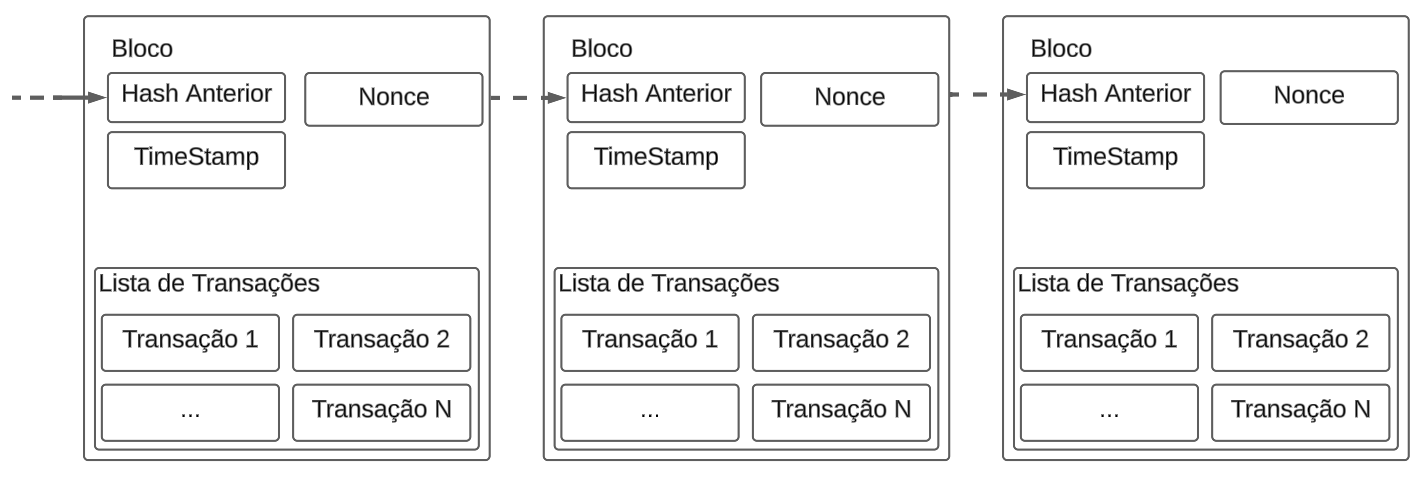
\includegraphics[width=.8\linewidth]{../images/figura 2.png}
	\label{fig:blockchain}
	\text{Fonte: Tradução pelos autores, baseado na documentação de referência \cite{Nakamoto2009}}
\end{figure}

Na Figura \ref*{fig:transactions} exibimos uma abstração da perspectiva do bloco, onde ocorre o encadeamento das transações seguido das suas respectivas assinaturas.

\begin{figure} [h]
	\centering
	\caption{Encadeamento das transações nos blocos.}
	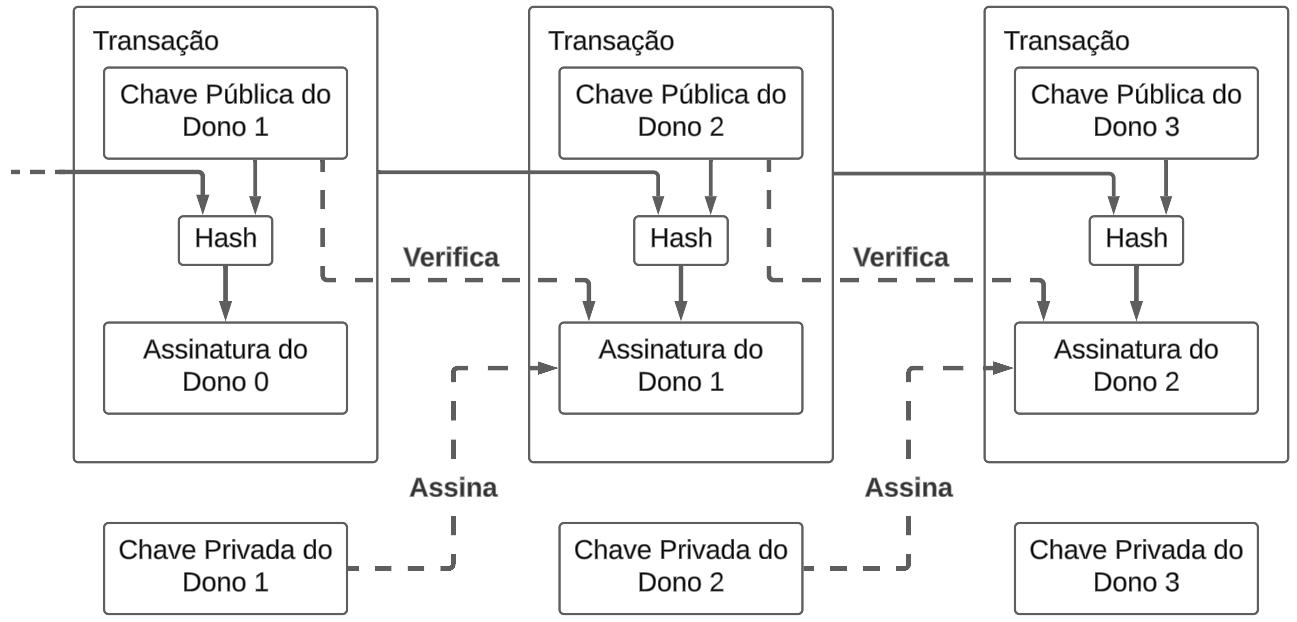
\includegraphics[width=.8\linewidth]{../images/figura 1.png}
	\label{fig:transactions}
	\text{Fonte: Tradução pelos autores, baseado na documentação de referência \cite{Nakamoto2009}}

\end{figure}

Em seguida é explicada a tecnologia de criptografia utilizada na atuação do \textit{Bitcoin}.

\section*{Criptografia SHA-256 (Secure Hash Algorithm 256-bit)} \label{subsec:sha256}
O protocolo do Bitcoin emprega a criptografia SHA-256 (\textit{Secure Hash Algorithm 256-bit}) como um componente fundamental para garantir a integridade e a segurança das transações na rede. Este algoritmo de \textit{hash} criptográfico, desenvolvido pela Agência Nacional de Segurança (NSA) dos Estados Unidos e publicado pelo Instituto Nacional de Padrões e Tecnologia (NIST), é crucial para diversas operações no ecossistema Bitcoin.

O SHA-256 contribui para a segurança geral do protocolo Bitcoin por ser resistente a ataques de colisão e de pré-imagem, o que significa ser computacionalmente impraticável encontrar duas mensagens distintas que resultem no mesmo \textit{hash} ou reverter um \textit{hash} para obter a mensagem original. Essas propriedades são essenciais para manter a integridade das chaves e transações, garantindo que as entradas não possam ser manipuladas sem que seja facilmente detectado pela rede.

\section*{Algoritmo de Prova de Trabalho e Mineiração} \label{subsec:pow}
Para garantir a segurança e a integridade da \textit{Blockchain}, o \textit{Bitcoin} utiliza um algoritmo de consenso chamado Prova de Trabalho (tambem chamado de \textit{Proof of Work} ou PoW). Os mineradores coletam transações pendentes em um bloco e tentam gerar um \textit{hash} válido para esse bloco usando o SHA-256.

A prova de trabalho se orienta dentro da \textit{blockchain} diante do protocolo Merkle. O protocolo Merkle, também referido como árvore de Merkle ou \textit{hash} de Merkle, é uma estrutura de dados fundamental em criptografia, criada por Ralph Merkle. A árvore de Merkle ajuda a garantir que os dados não foram alterados, pois, qualquer modificação nos dados de entrada alteraria o \textit{hash} na folha correspondente e, por sua vez, todos os \textit{hashes} no caminho até a raiz.


O algoritmo é aplicado duas vezes (conhecido como \textit{double-SHA-256}) ao cabeçalho do bloco, que inclui a versão do programa, o \textit{hash} do bloco anterior, o \textit{hash} Merkle das transações no bloco, o \textit{timestamp}, o nível de dificuldade e um \textit{nonce}. O termo \textit{nonce} refere-se a um número que é usado apenas uma vez (do inglês \textit{number used once}). O \textit{nonce} é um valor inteiro de 32 bits que os mineradores ajustam repetidamente para tentar produzir um \textit{hash} do bloco que atenda aos critérios de dificuldade estabelecidos pela rede Bitcoin.

O objetivo é encontrar um \textit{hash} que seja menor que o valor de dificuldade estabelecido pela rede, o que exige que os mineradores ajustem o \textit{nonce} repetidamente e recalculam o \textit{hash} do bloco até que um valor adequado seja encontrado. Este processo é fundamental para a implementação da prova de trabalho (\textit{Proof of Work} - PoW), que ajuda a proteger a rede contra ataques.

\clearpage
\section{Escola Austríaca de Economia} \label{sec:austriaca}
A Escola Austríaca de Economia, emergida no final do século XIX, representa uma tradição heterodoxa significativa no pensamento econômico. Caracterizada por sua ênfase na teoria subjetiva do valor, na praxeologia e no papel crucial do empreendedorismo, a Escola Austríaca oferece uma perspectiva única que contrasta com as abordagens neoclássicas e keynesianas dominantes.

Seguidamente é revisitada a história, cronologia, os principais autores e pautas centrais desta escola, destacando suas contribuições teóricas e influências duradouras. É constatado também definições por parte destes autores diante dos conceitos, respectivamente, de economia, capital e dinheiro

% \section*{Origens}

A Escola Austríaca de Economia foi fundada por Carl Menger com a publicação de \textit{"Principles of Economics"} (1871). Seu trabalho desafiou a teoria do valor-trabalho dos economistas clássicos e introduziu a teoria marginalista do valor.

\section*{Carl Menger (1840-1921)}
Em \textit{"Principles of Economics"}, \cite{menger1871principles} argumentou que o valor dos bens é determinado pela utilidade marginal que os indivíduos o atribuem, estabelecendo as bases para a análise econômica subjetiva.

\section*{Eugen von Böhm-Bawerk (1851-1914)}
Discípulo de Menger, Böhm-Bawerk contribuiu significativamente para a teoria do capital e dos juros. Em \textit{"Capital and Interest"}, ele desenvolveu a teoria da estrutura temporal da produção, enfatizando a importância do tempo no processo produtivo \cite{bohm1884capital}.

\section*{Friedrich von Wieser (1851-1926)}
Wieser é conhecido por sua teoria do custo de oportunidade e pelo desenvolvimento da teoria do valor imputado. Ele ajudou a consolidar a Escola Austríaca como uma corrente de pensamento econômico significativa \cite{bohm1884capital}.

\section*{Desenvolvimento e Consolidação}

No início do século XX, Ludwig von Mises e Friedrich Hayek ampliaram e consolidaram as ideias da Escola Austríaca, influenciando significativamente o pensamento econômico.

\section*{Ludwig von Mises (1881-1973)}
Mises é uma figura central na Escola Austríaca. Em \textit{"Human Action"}, ele propôs que a economia deve ser baseada na lógica dedutiva da ação humana, uma abordagem chamada praxeologia. Mises também desenvolveu a teoria do ciclo econômico, que analisa as flutuações econômicas causadas pela expansão do crédito e pela intervenção estatal no mercado monetário \cite{mises1949human}.

\section*{Friedrich Hayek (1899-1992)}
Discípulo de Mises, Hayek contribuiu para a teoria do capital e o estudo dos ciclos econômicos. Em \textit{"The Road to Serfdom"} e \textit{"The Constitution of Liberty"}, Hayek criticou o intervencionismo estatal e defendeu uma ordem espontânea de mercado. Em 1974, ele recebeu o Prêmio Nobel de Economia por seu trabalho sobre a teoria monetária e as flutuações econômicas \cite{hayek1944road},\cite{hayek1960constitution}.

\section*{Expansão e Influência Contemporânea}

Na segunda metade do século XX e início do século XXI, a Escola Austríaca continuou a evoluir com novos pensadores que expandiram suas teorias e influências.

\section*{Murray Rothbard (1926-1995)}
Rothbard combinou a economia austríaca com uma filosofia libertária. Em \textit{"Man, Economy, and State"}, ele apresentou uma visão abrangente da economia austríaca e criticou a intervenção estatal. \cite{rothbard1962man}.

\section*{Israel Kirzner (1930-)}
Kirzner contribuiu para a teoria do empreendedorismo, destacando o papel do empreendedor na descoberta de oportunidades de mercado e na coordenação econômica. Seu trabalho \textit{"Competition and Entrepreneurship"} é uma referência importante para o estudo do processo de mercado e da função empresarial \cite{kirzner1973competition}.

\section*{Pautas e Contribuições}
A seguir consta as principais pautas da Escola Austríaca aonde servirá de base para o relacionamento dos conceitos fundamentais de economia, dinheiro e capital.

\section*{Teoria do Valor Subjetivo}

A teoria do valor subjetivo é uma contribuição fundamental da Escola Austríaca. Ela afirma que o valor dos bens é determinado pela utilidade marginal atribuída pelos indivíduos, contrastando com a teoria do valor-trabalho \cite{menger1871principles}.

\section*{Praxeologia}

A praxeologia é a metodologia central da Escola Austríaca. Baseia-se na premissa de que a economia é uma ciência social que deve ser estudada através da análise lógica da ação humana, ao invés de métodos empíricos e estatísticos \cite{mises1949human}.

\section*{Teoria do Ciclo Econômico}

A teoria austríaca do ciclo econômico, desenvolvida por Mises e Hayek, explica as flutuações econômicas como resultado das distorções causadas pela expansão do crédito e pela intervenção governamental. Segundo esta teoria, a criação artificial de crédito leva a um mau investimento de recursos, resultando em ciclos de \textit{boom} e \textit{bust} \cite{mises1949human,hayek1944road}.

\section*{Crítica ao Intervencionismo Estatal}

A Escola Austríaca é fortemente crítica ao intervencionismo estatal e ao planejamento centralizado. Economistas austríacos argumentam que a intervenção governamental distorce os sinais de preço, leva a alocações ineficientes de recursos e restringe a liberdade individual. Hayek argumentou que o planejamento centralizado é incapaz de lidar com a complexidade da informação distribuída na sociedade \cite{hayek1944road,hayek1960constitution}.

\section*{Teoria do Empreendedorismo}

A ênfase no papel do empreendedor é uma característica distintiva da Escola Austríaca. Kirzner destacou que os empreendedores são essenciais para a descoberta e exploração de oportunidades de mercado, contribuindo para a coordenação econômica e a dinâmica dos mercados \cite{kirzner1973competition}.

\section{Definição conceitual de maior incisão no projeto}

Consta aqui definições por parte dos autores austríacos diante dos conceitos de base da atuação deste artigo. A partir desta conceitualização é possível observar diante da atuação dos criptoativos e futuramente estipular as necessidades de um sistema de moedas digitais, dedicado ao ensino de finanças.

\section*{Economia e a Ação Humana}
Ludwig von Mises, em "Ação Humana"\cite{mises1949human}, define economia como "a ciência que estuda a ação humana, uma aplicação da teoria do conhecimento humano". Segundo Mises, a economia é um ramo da praxeologia, ou seja, a teoria da ação humana. Ele argumenta que a economia, ao contrário de ser meramente uma análise de dados e tendências, é fundamentalmente sobre como os indivíduos escolhem agir com recursos escassos para atingir seus objetivos.

\section*{Capital segundo Böhm-Bawerk}
Eugen Böhm von Bawerk, contribuiu significativamente para a teoria do capital. Em sua obra \textit{"Capital and Interest"}\cite{bohm1884capital}, Böhm-Bawerk descreve o capital como "bens produzidos que servem como meios para a aquisição de bens futuros" \cite{bohm1884capital}. Ele esclarece que o capital não é simplesmente uma acumulação de dinheiro ou ativos, mas sim ferramentas, máquinas e materiais usados para aumentar a produção futura.

\section*{Dinheiro e sua Origem para Menger}
Carl Menger, foi um dos primeiros economistas a explicar a origem do dinheiro através de um processo de evolução social e não por decreto governamental ou convenção. Em sua obra "Princípios de Economia Política" \cite{menger2017liberalismo}, Menger argumentou que o dinheiro emergiu organicamente como o meio mais vendável de troca, facilitando assim as transações comerciais e reduzindo os custos de transação na economia \cite{menger1871principles}.

\section*{Hayek e a Desestatização do Dinheiro}
Friedrich Hayek, levou a teoria monetária austríaca para outra direção ao argumentar a favor da competição de moedas privadas em sua obra "Desnacionalização do Dinheiro" \cite{hayek2017desestatizaccao}. Hayek criticou os monopólios governamentais sobre a emissão de dinheiro, propondo que a concorrência entre diferentes categorias de dinheiro poderia prevenir a inflação e promover a estabilidade econômica.

\section*{A Teoria do Dinheiro de Mises}
Ludwig von Mises expandiu a teoria de Menger ao introduzir o conceito de "regressão" em sua análise do valor do dinheiro. Em "A Teoria do Dinheiro e do Crédito" \cite{von2013theory}, Mises apresenta a ideia de que o valor do dinheiro hoje é derivado da expectativa de seu poder de compra no futuro, que por sua vez é baseado em uma regressão contínua até o ponto em que o dinheiro era apenas um bem mais vendável entre outros \cite{von2013theory}. Mises também destacou o papel do dinheiro no cálculo econômico, essencial para a alocação racional de recursos em uma economia de mercado.

\section*{Rothbard e a Crítica à Moeda Fiduciária}
Murray Rothbard, seguindo a indução de Mises, foi crítico em relação ao sistema de moeda fiduciária e ao papel dos bancos centrais. Em "O que o Governo fez com o Nosso Dinheiro?" \cite{rothbard2022governo}, Rothbard explica como o dinheiro historicamente ancorado em commodities, como o ouro, foi progressivamente substituído por dinheiro papel sem lastro, levando a ciclos econômicos mais instáveis e inflação.

\section{Bitcoin é dinheiro de verdade?} \label{sec:dinheiro}
Nesta secção, fazemos uma revisão do livro "\textit{Bitcoin}, a moeda na era digital"\cite{Ulrich2014} escrito por Fernando Ulrich. O brasileiro é Mestre em Economia e referência por seu pioneirismo na divulgação de criptomoedas no Brasil.

\section*{Definição de Ulrich de Dinheiro e Moeda}
Em seu livro, Ulrich chega a definição de moeda como "qualquer bem econômico empregado indefinidamente como meio de troca, independentemente de sua liquidez frente a outros bens monetários e de seus possíveis usos alternativos" \cite[P.89]{Ulrich2014}.

O autor lista atributos característicos a moeda, sendo eles sua escassez,
durabilidade, homogeneidade espacial e temporal, divisibilidade e maleabilidade, comparando o desempenho destes atributos diante do papel-moeda, o ouro e o Bitcoin, como mostra na Tabela \ref*{tab:atributos}.

% \begin{figure} [h]
% 	\centering
% 	\caption{Comparação dos atributos do dinheiro diante do ouro, do papel-moeda e do \textit{Bitcoin}}
% 	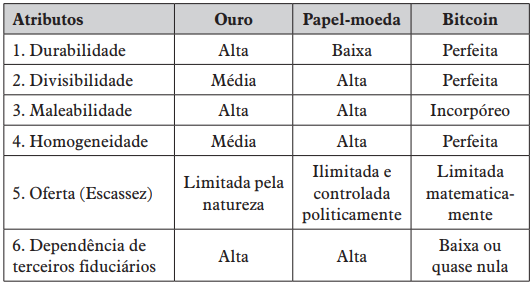
\includegraphics[width=.8\linewidth]{images/atributos.png}
% 	\label{fig:atributos}
% 	\text{Fonte: \cite[p.67]{Ulrich2014}.}
% \end{figure}
% Please add the following required packages to your document preamble:
% \usepackage[table,xcdraw]{xcolor}
% Beamer presentation requires \usepackage{colortbl} instead of \usepackage[table,xcdraw]{xcolor}
\FloatBarrier
\begin{table}[h]
    \centering
	\caption{Comparação dos atributos do dinheiro diante do ouro, do papel-moeda e do \textit{Bitcoin}}.
	\begin{tabular}{|c|c|c|c|}
        
		\hline
		\rowcolor[HTML]{C0C0C0}
		\textbf{Atributos}                                                                & \textbf{Ouro}                                                     & \textbf{Papel-moeda}                                                              & \textbf{Bitcoin}                                                    \\ \hline
		1.Durabilidade                                                                    & Alta                                                              & Baixa                                                                             & Perfeita                                                            \\ \hline
		2.Divisibilidade                                                                  & Média                                                             & Alta                                                                              & Perfeita                                                            \\ \hline
		3.Maleabilidade                                                                   & Alta                                                              & Alta                                                                              & Incorpóreo                                                          \\ \hline
		4.Homogeneidade                                                                   & Média                                                             & Alta                                                                              & Perfeita                                                            \\ \hline
		5.Oferta(Escassez)                                                                & \begin{tabular}[c]{@{}c@{}}Limitada pela \\ natureza\end{tabular} & \begin{tabular}[c]{@{}c@{}}Limitada e \\ controlada \\ politicamente\end{tabular} & \begin{tabular}[c]{@{}c@{}}Limitada \\ Matematicamente\end{tabular} \\ \hline
		\begin{tabular}[c]{@{}c@{}}6.Dependência de \\ terceiros fiduciários\end{tabular} & Alta                                                              & Alta                                                                              & \begin{tabular}[c]{@{}c@{}}Baixa ou \\ quase nula\end{tabular}      \\ \hline
	\end{tabular}
    \label{tab:atributos}
\end{table}
\FloatBarrier

Ulrich menciona também as funções do dinheiro, listadas de servir como meio de troca, reserva de valor e unidade de conta. Em outras palavras, uma moeda deve servir, respectivamente, de maneira que as suas trocas sejam de forma facilitada; deve atuar de maneira em que possa ser entesourada e/ou guardada como reserva de riqueza; e por fim permita ser utilizável como meio de conta, utilizável ao cálculo econômico em função da moeda.

Segundo Fernando, o \textit{Bitcoin} mostra-se capaz de performar as características e as funções da moeda tão bem, se não melhor, que o ouro e o papel-moeda. De acordo com ele "apesar da aparência unicamente digital, as atuais formas de dinheiro assemelham-se em muito ao \textit{Bitcoin}. A maior parte da massa monetária no mundo moderno manifesta-se de forma intangível; nosso dinheiro já é um bem incorpóreo, uma característica que em nada nos impede de usá-lo diariamente"\cite[p.95]{Ulrich2014}.



% \section*{DESENVOLVIMENTO}
\chapter{Conceito de possível aplicação da arquitetura de criptoativos}

\section*{Um criptoativo educativo}
\label{sec:educativo}











\section*{CONCLUSÃO}
Neste projeto, percorremos por meio do contexto técnico e social do desenvolvimento dos criptoativos, averiguamos a motivação de desintermediação das atividades financeiras por meio da origem do \textit{Bitcoin}; exploramos o ecossistema cripto por meio dos contratos inteligentes e da \textit{DeFi}, e exibimos seu impacto diante da economia tradicional.

Sob maior incisão teórica no projeto, apresentamos os conceitos chave do funcionamento do \textit{Bitcoin}, constatamos a estrutura dos blocos, a estrutura do encadeamento, o procedimento de prova de trabalho utilizado na mineração do \textit{Bitcoin} e como constitui o seu caráter criptográfico.

Apresentamos também como a natureza do \textit{Bitcoin}, de maneira programática, corrobora aos conceitos técnico-economicos da Escola Austríaca de Economia, provendo respaldo diante das características do dinheiro, tão bem como as funções da moeda. Apresentamos o resultado da comparação de suas características ao papel-moeda e ao ouros por Fernando Ulrich.

Por fim, atuamos na experimentação educacional da implementação de um sistema de \textit{blockchain} de nível médio, que abstrai os conceitos base do \textit{Bitcoin}, permite a manipulação via requisições e exibe as classes presentes da corrente no navegador. Apresentamos todas as estruturas geradas neste experimento, seus atributos e suas funções diantes da rede.

\section*{Exibição do Experimento de \textit{Blockchain} em Rust}
Nas Figuras a seguir constam as imagens desta experimentação, o repositório onde o código e os arquivos deste teste foram armazenados na plataforma Github por preferência dos autores. O código se encontra disponível por este link:
\href{https://github.com/HeberUnifil/Educational-Blockchain-Currency}{\textcolor{blue}{https://github.com/HeberUnifil/Educational-Blockchain-Currency}} .

Na Figura \ref*{fig:terminal} consta o registro via terminal Linux das atualizações realizadas na \textit{Blockchain}:

\begin{figure} [h]
	\centering
	\caption{Resposta via terminal sobre as atualizações na \textit{Blockchain}.}
	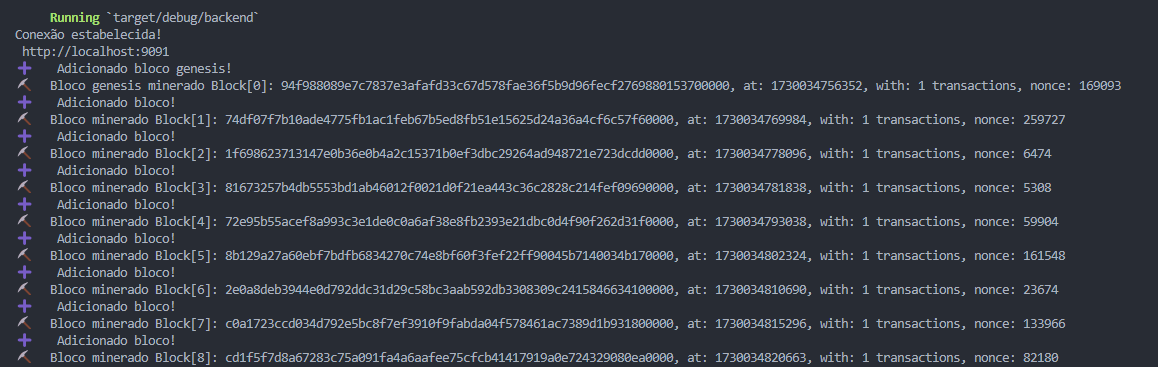
\includegraphics[width=.8\linewidth]{../images/terminal-blockchain.png}
	\label{fig:terminal}
	\text{Fonte: Captura de tela tirada pelos autores}

\end{figure}

Na Figura \ref*{fig:navegador} consta a exibição geral dos blocos ordenados na corrente, seus respectivos \textit{hashes}, sua marca temporal, quantidade de transações e o número de tentativas para mineração do bloco.

\begin{figure} [h]
	\centering
	\caption{Resposta via terminal sobre as atualizações na \textit{Blockchain}.}
	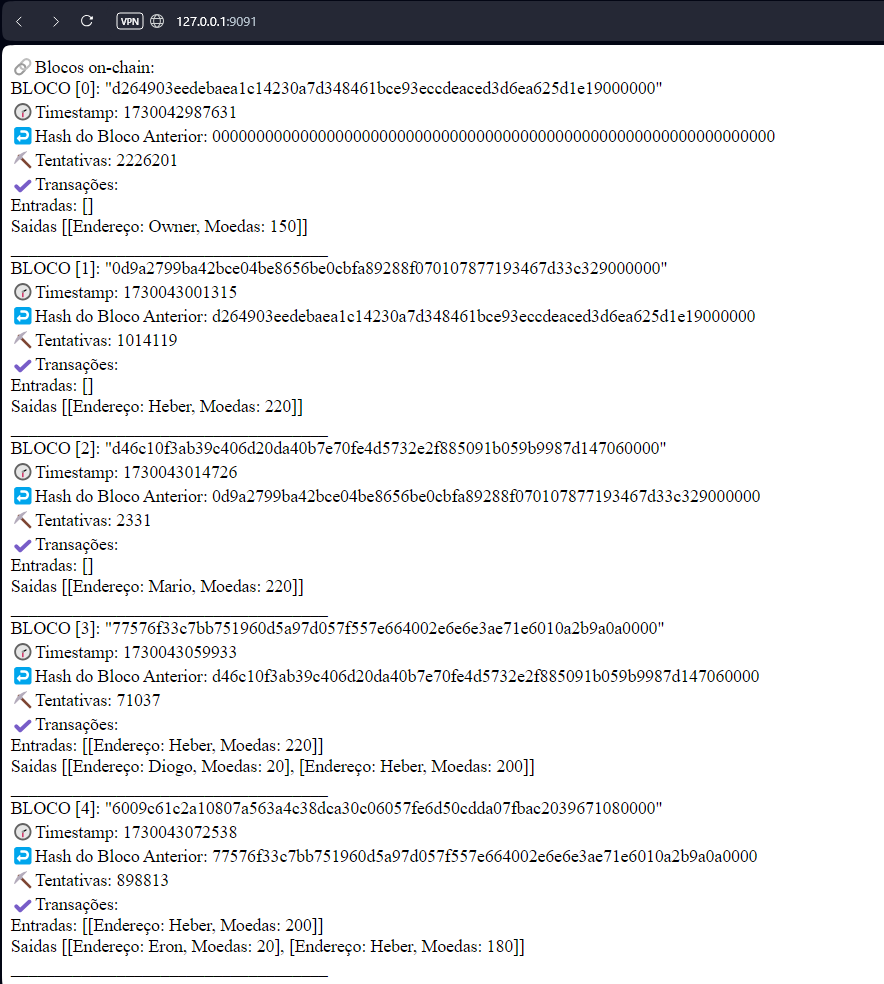
\includegraphics[width=.8\linewidth]{../images/navegador-blockchain.png}
	\label{fig:navegador}
	\text{Fonte: Captura de tela tirada pelos autores}

\end{figure}

% \begin{figure} [h]
% 	\centering
% 	\caption{Resposta via terminal sobre as atualizações na \textit{Blockchain}.}
% 	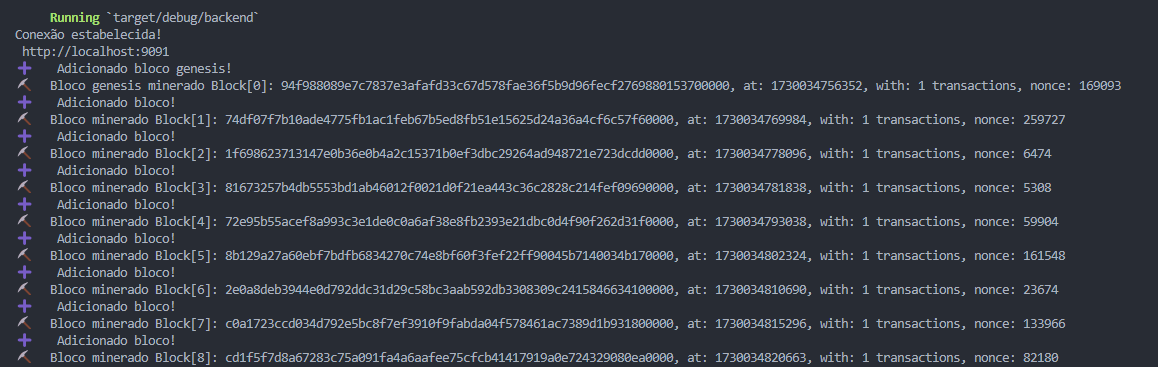
\includegraphics[width=.8\linewidth]{../images/terminal-blockchain.png}
% 	\label{fig:terminal}
% 	\text{Fonte: Captura de tela tirada pelos autores}

% \end{figure}

\end{Spacing}
\postextual

% bibliografia %
\bibliography{bibliografia}

\end{document}